%%%%%%%%%%%%%%%%%%%%%%%%%%%%%%%%%%%%%%%%%
% baposter Portrait Poster
% LaTeX Template
% Version 1.0 (15/5/13)
%
% Created by:
% Brian Amberg (baposter@brian-amberg.de)
%
% This template has been downloaded from:
% http://www.LaTeXTemplates.com
%
% License:
% CC BY-NC-SA 3.0 (http://creativecommons.org/licenses/by-nc-sa/3.0/)
%
%%%%%%%%%%%%%%%%%%%%%%%%%%%%%%%%%%%%%%%%%

%----------------------------------------------------------------------------------------
%	PACKAGES AND OTHER DOCUMENT CONFIGURATIONS
%----------------------------------------------------------------------------------------

\documentclass[a0paper,portrait]{baposter}

\usepackage[font=small,labelfont=bf]{caption} % Required for specifying captions to tables and figures
\usepackage{booktabs} % Horizontal rules in tables
\usepackage{relsize} % Used for making text smaller in some places

\usepackage{paralist}
\usepackage{wrapfig}
\usepackage{arabtex}
\usepackage[font=normalsize,labelfont=sf,textfont=sf]{subfig}
\usepackage{graphicx}
\usepackage{xcolor,colortbl}
\usepackage[cmex10]{amsmath}
\usepackage{sidecap}
\usepackage{eufrak}
\usepackage{amssymb}



\usepackage[pscoord]{eso-pic}% The zero point of the coordinate systemis the lower left corner of the page (the default).

\newcommand{\placetextbox}[3]{% \placetextbox{<horizontal pos>}{<vertical pos>}{<stuff>}
  \setbox0=\hbox{#3}% Put <stuff> in a box
  \AddToShipoutPictureFG*{% Add <stuff> to current page foreground
    \put(\LenToUnit{#1\paperwidth},\LenToUnit{#2\paperheight}){\vtop{{\null}\makebox[0pt][c]{#3}}}%
  }%
}%

\graphicspath{{figures/}} % Directory in which figures are stored

\definecolor{bordercol}{RGB}{79,129,189} % Border color of content boxes
\definecolor{headercol1}{RGB}{55,96,146} % Background color for the header in the content boxes (left side)
\definecolor{headercol2}{RGB}{55,96,146} % Background color for the header in the content boxes (right side)
\definecolor{headerfontcol}{RGB}{237,237,237} % Text color for the header text in the content boxes
%\definecolor{boxcolor}{RGB}{186,215,230} % Background color for the content in the content boxes
\definecolor{boxcolor}{RGB}{252,252,252} % Background color for the content in the content boxes


\definecolor{IceBlue}{RGB}{233,237,244}
\definecolor{IceBlue2}{RGB}{208,216,232}

\begin{document}

\background{ % Set the background to an image (background.pdf)
\begin{tikzpicture}[remember picture,overlay]
\draw (current page.north west)+(-0.3em,0.3em) node[anchor=north west]
{
\includegraphics[height=0.1\textheight, width=1.07\textwidth]{title_back}};
\end{tikzpicture}
}

\begin{poster}{
grid=false,
borderColor=bordercol, % Border color of content boxes
headerColorOne=headercol1, % Background color for the header in the content boxes (left side)
headerColorTwo=headercol2, % Background color for the header in the content boxes (right side)
headerFontColor=headerfontcol, % Text color for the header text in the content boxes
boxColorOne=boxcolor, % Background color for the content in the content boxes
headershape=roundedright, % Specify the rounded corner in the content box headers
headerfont=\Large\sf\bf, % Font modifiers for the text in the content box headers
textborder=rectangle,
background=user,
headerborder=open, % Change to closed for a line under the content box headers
boxshade=plain
}
{}
%
%----------------------------------------------------------------------------------------
%	TITLE AND AUTHOR NAME
%----------------------------------------------------------------------------------------
%
{\sf\bf\color{white} Real-time Segmentation of On-line\\Handwritten Arabic Script}
{\vspace{0.1em}\color{white} George Kour$^1$, Raid Saabni$^2$ \\ 
{\smaller $^1$Faculty of Engineering, Tel-Aviv University, Israel} \\
{\smaller $^2$Triangle R\&D Center, Kafr Qara, Israel}}

\placetextbox{0.95}{0.98}{\includegraphics[width=0.07\linewidth]{tau}}
\placetextbox{0.07}{0.97}{\includegraphics[width=0.12\linewidth]{trc}}

%----------------------------------------------------------------------------------------
%	INTRODUCTION
%----------------------------------------------------------------------------------------

\headerbox{Introduction}{name=introduction,column=0,row=0}{
Delaying the analysis launch until the completion of the word scribing:
\begin{compactenum}
\item Limit responsiveness.
\item Prevent implementing advanced features of input typing, such as Automatic word completion \& Real-time automatic spelling.\\
\end{compactenum}

However, conventional approaches usually wait until the entire curve is traced out before starting the analysis, inevitably causing delays in the recognition process. \\

\textbf{We propose a real-time recognition-based segmentation technique of on-line Arabic script.
It demonstrates the feasibility of carrying out the most time consuming tasks, required for the segmentation process, during the course of writing.\\}

The real-time segmentation and classification information can be used to significantly reduce the potential dictionary size and accelerate a later holistic recognition process.

}

%----------------------------------------------------------------------------------------
%	THE ADAB DATASET
%----------------------------------------------------------------------------------------

\headerbox{The ADAB database}{name=dataset,column=0,below=introduction}{
The system was trained and tested on samples taken from the ADAB database.
It consists of more than 20k Arabic on-line handwritten words (937 Tunisian town/village names) scribed by more than 170 different writers.
However, the ADAB only provides the strokes data for a given sample.
\vspace{-5pt}
\begin{center}
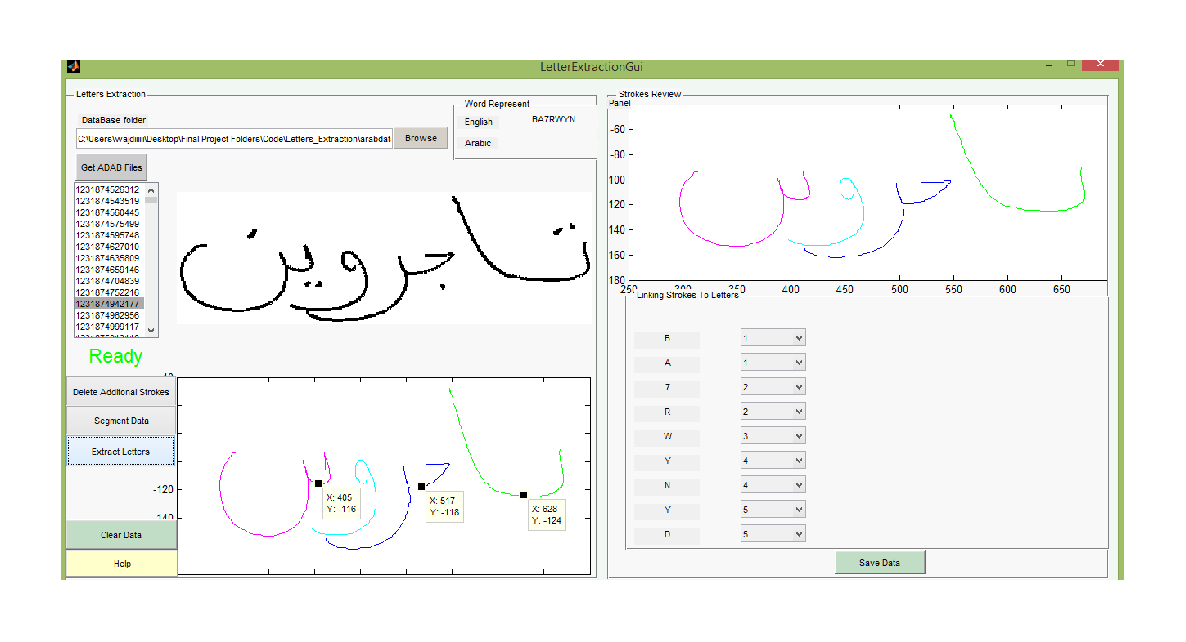
\includegraphics[width=0.7\linewidth]{letter_extraction_gui}
\vspace{-10pt}
\captionof{figure}{Manual segmentation of ADAB sample into: Word-Pars (WPs), Strokes and Letters.}
\end{center}

\textbf{We are planning to standardize and publish the data extracted from the ADAB database.}

\begin{center}
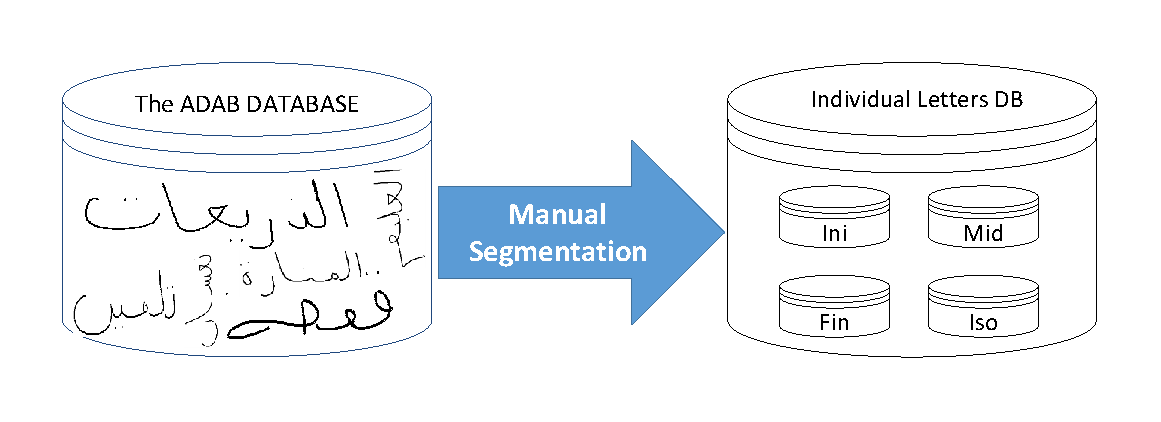
\includegraphics[width=1\linewidth]{adab_segmentation}
\vspace{-25pt}
\captionof{figure}{The letters samples were split to four databases according to their position.}
\end{center}

\begin{center}
\captionof{table}{Individual characters training set distribution.}
\begin{tabular}{c c}
\toprule
\textbf{Letter Position} & \textbf{\# of samples}\\
\midrule
\rowcolor{IceBlue}
Ini & 1405 \\
\rowcolor{IceBlue2}
Mid & 1196 \\
\rowcolor{IceBlue}
Fin & 1629 \\
\rowcolor{IceBlue2}
Iso & 1372 \\
\bottomrule
\end{tabular}
\end{center}

\begin{center}
\captionof{table}{System testing set information.}
\begin{tabular}{ c  c }
  \rowcolor{IceBlue}
  \# of city names & 319 \\
  \rowcolor{IceBlue2}
  \# of WPs & 1148 \\
  \rowcolor{IceBlue}
  \# of strokes & 1237 \\
\end{tabular}
\end{center}
}


%----------------------------------------------------------------------------------------
%	System Overview 1
%----------------------------------------------------------------------------------------

\headerbox{System Overview}{name=overview,span=1,column=1,row=0}{ % To reduce this block to 1 column width, remove 'span=2'

\begin{center}
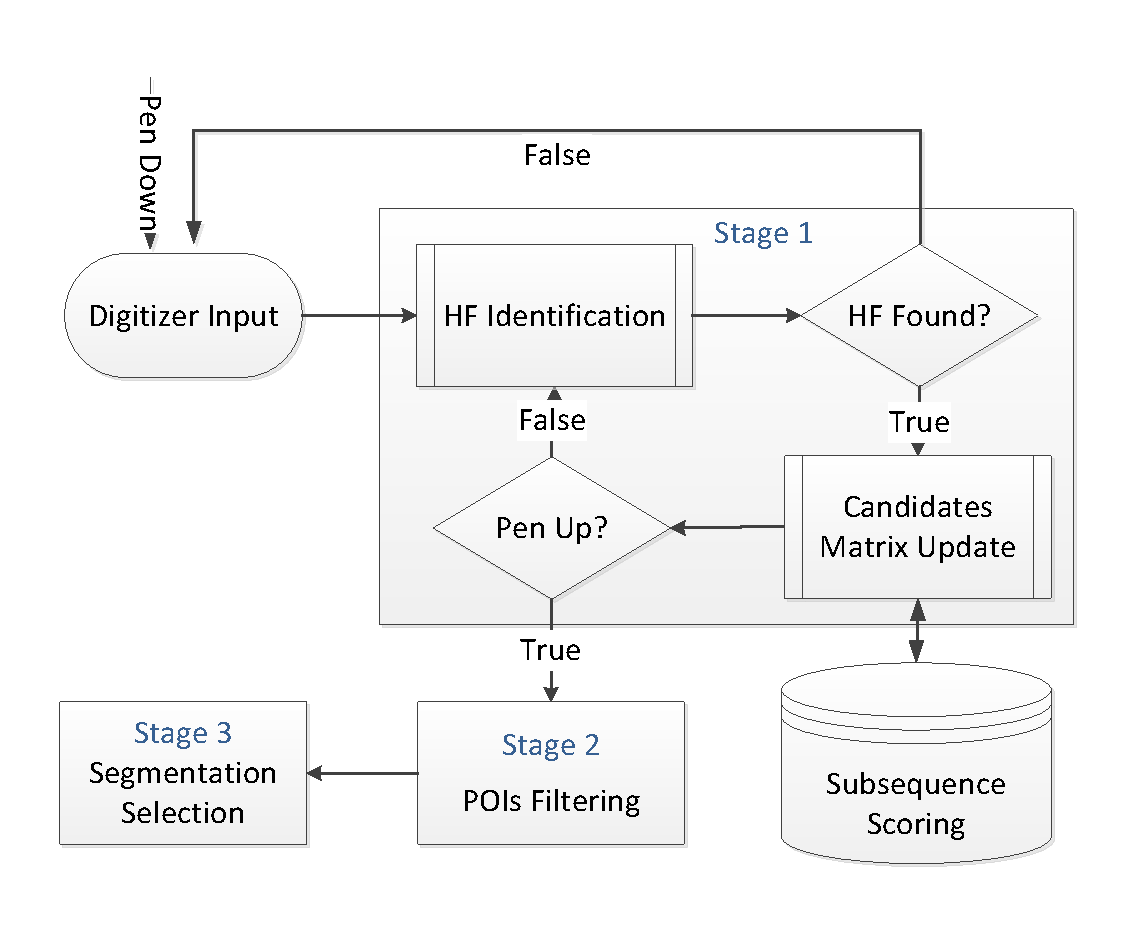
\includegraphics[width=1\linewidth]{system_flow}
\end{center}

}

%----------------------------------------------------------------------------------------
%	Stage 1
%----------------------------------------------------------------------------------------

\headerbox{Stage 1}{name=stage1,span=1,column=2,row=0}{ 
\emph{Points of interest} (POIs), i.e., potential segmentation points (SPs), are continuously nominated using morphological features \textbf{while the stroke is being scribed}.

\vspace{-15pt}
\begin{center}
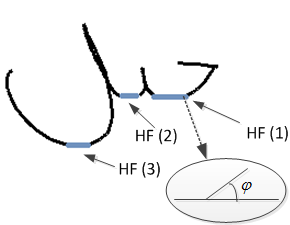
\includegraphics[width=0.6\linewidth]{horizontal_fragments}
\vspace{-15pt}
\captionof{figure}{\emph{Horizontal Fragments} (HFs) are ligatures that join pairs of connected letters in the Arabic script are usually horizontal, directed right to left and located near the baseline. POIs are the mid-points of HFs.}
\end{center}

\vspace{-25pt}
\begin{center}
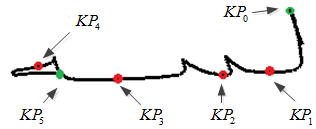
\includegraphics[width=0.8\linewidth]{candidate_points}
\vspace{-15pt}
\captionof{figure}{The KPs (Key-Points) set is the ordered set of POIs, in addition to the first and the last points of the stroke positioned as the first and the last items in the set }
\end{center}

The classification information of the sub-strokes imposed by the KPs is stores in a matrix like data structure, $D$, where each cell $D_{i,j}$ contains the scoring information for the sub-strokes $S_i^j$. 

{\smaller
\begin{center}
\renewcommand{\arraystretch}{1.1}
\begin{tabular}{ c | c  c  c  c  c }
%\hline
\toprule
     & $1$ & $2$ & $3$ & $4$ & $5$ \\
%\hline
\midrule
$0$
   & 
\includegraphics[width=0.13\linewidth]{./figures/substrokes/L}
   & 
\includegraphics[width=0.13\linewidth]{./figures/substrokes/LB1}
   & 
\includegraphics[width=0.13\linewidth]{./figures/substrokes/LB1B2}
   & $\varnothing$ & $\varnothing$ \\
%\hline
$1$
   & $\varnothing$
   & 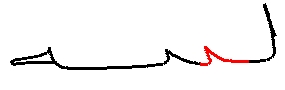
\includegraphics[width=0.13\linewidth]{./figures/substrokes/B1}
   & 
\includegraphics[width=0.13\linewidth]{./figures/substrokes/B1B2}
   & 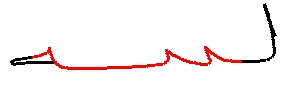
\includegraphics[width=0.13\linewidth]{./figures/substrokes/B1B2H1}
   & $\varnothing$ \\
%\hline
$2$
   & $\varnothing$  & $\varnothing$
   & 
\includegraphics[width=0.13\linewidth]{./figures/substrokes/B2}
   & 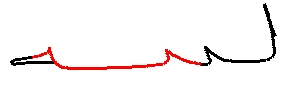
\includegraphics[width=0.13\linewidth]{./figures/substrokes/B2H1}
   & 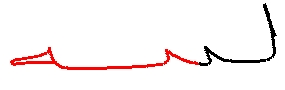
\includegraphics[width=0.13\linewidth]{./figures/substrokes/B2H} \\
%\hline
$3$
   & $\varnothing$ & $\varnothing$ & $\varnothing$ 
   & 
\includegraphics[width=0.13\linewidth]{./figures/substrokes/H1}
   & 
\includegraphics[width=0.13\linewidth]{./figures/substrokes/H} \\
%\hline
$4$
   & $\varnothing$ & $\varnothing$ & $\varnothing$ & $\varnothing$ 
   & 
\includegraphics[width=0.13\linewidth]{./figures/substrokes/H2}\\
%\hline
\bottomrule
\end{tabular}
\captionof{figure}{The $D$ matrix.}
\end{center}
}
}

%----------------------------------------------------------------------------------------
%	Stage 2
%----------------------------------------------------------------------------------------

\headerbox{Stage 2}{name=stage2,span=1,column=2,row=0,below=stage1}{ 

Once the entire stroke is available, a rules-based process is used to refine the set of POIs and re-score the sub-strokes based on the following rules: 
\begin{compactitem}
\item SPs should lie close to the baseline. 
\item do not reside in loops.
\item sub-stroke length should be proportional to the length of the containing stroke.	
\end{compactitem}

}

%----------------------------------------------------------------------------------------
%	Stage 3
%----------------------------------------------------------------------------------------

\headerbox{Stage 3}{name=stage3,span=1,column=2,below=stage2}{ 
The goal of this phase is to select the \emph{final segmentation points} (FSP) set among the POIs.

One can model the matrix $D$ as a directed, edge-weighted graph $G=(V,E)$, for which a path from vertex $KP_0$ to vertex $KP_{L+1}$ defines a possible segmentation.

\vspace{-10pt}
\begin{center}
\captionof{table}{Segmentation path selection performance.}
\vspace{-10pt}
\begin{tabular}{c c c c}
\hline
\toprule
\textbf{Alg.} & \textbf{WP SR}  &\textbf{SP Pre.} & \textbf{SP Rec.}\\
\midrule
  \rowcolor{IceBlue}             
  FSS & 76\% & 85\% & 78\% \\ 
  \rowcolor{IceBlue2}
  BSS & 79\% & 84\%& 81\% \\
  \rowcolor{IceBlue}
  BFSS & 78\%  & 84\% & 80\%\\ 
  \rowcolor{IceBlue2}
  GSS & 80\% & 81\% & \bf{94}\% \\  
  \rowcolor{IceBlue}
  FSS$\oplus$BSS & \bf{82}\%  & \bf{89}\% & 82\%\\  
  \bottomrule
\end{tabular}
\end{center}

}

%----------------------------------------------------------------------------------------
%	RESULTS
%----------------------------------------------------------------------------------------

\headerbox{Results}{name=results,span=1,column=1,below=overview}{ 

\begin{center}
\captionof{table}{System Segmentation Accuracy.}
\vspace{-10pt}
\begin{tabular}{cc||cc}
  %\toprule
  \rowcolor{IceBlue}
  Strokes SR &  83\% & Missing SPs  & 14.7\%\\
  \rowcolor{IceBlue2}
  Strokes RR &  78\% & Invalid SPs  & 11\%\\
  \rowcolor{IceBlue}
  \# true SPs & 1081 & SPs precision & 88.6\%\\ 
  \rowcolor{IceBlue2}
  Valid SPs  & 85.3\% & SPs recall  &  85.3\%\\
  %\bottomrule
\end{tabular}
SR - Segmentation rate; RR - Recognition rate;
\end{center}

\textbf{Over-segmentation:}
\begin{compactitem}
\item A horizontal region in initial form which does not accommodate a SP.
\item A letter spanned over several strokes.
\end{compactitem}

\textbf{Under-segmentation:}
\begin{compactitem}
\item Letter pairs that are not separated by HFs (e.g., \RL{lm} and \RL{l.h} ).
\item Not selecting a POI in the third stage.\\
\end{compactitem}

\textbf{Holistic WPs Recognition:}
\begin{compactenum}
\item Take the $10$ top scored candidates of the sub-strokes.
\item Generate a complete list of all possible shape concatenation of the retrieved candidates. 
\item Holistic match against the queried WP.  
\end{compactenum}
\vspace{-15pt}
\begin{center}
\captionof{table}{Holistic WPs Recognition Results.}
\begin{tabular}{c c}
\toprule
\textbf{\# Top Candidates } & \textbf{WP RR}\\
\midrule
\rowcolor{IceBlue}
$1$ & $90.8\%$ \\
\rowcolor{IceBlue2}
$5$ & $94.7\%$ \\
\rowcolor{IceBlue}
$10$ & $98.1\%$ \\
\bottomrule
\end{tabular}
\end{center}


}

%----------------------------------------------------------------------------------------
%	RESULTS
%----------------------------------------------------------------------------------------

\headerbox{Characters Sample Set}{name=letters_dist,span=1,column=1,below=results}{ 

The characters in the ADAB database is from a limited dictionary, thus, the character samples distribution is imbalanced. 

We measured the effect of a large and imbalanced characters training set on the WP SR and RR. 

%\vspace{-10pt}
\begin{center}
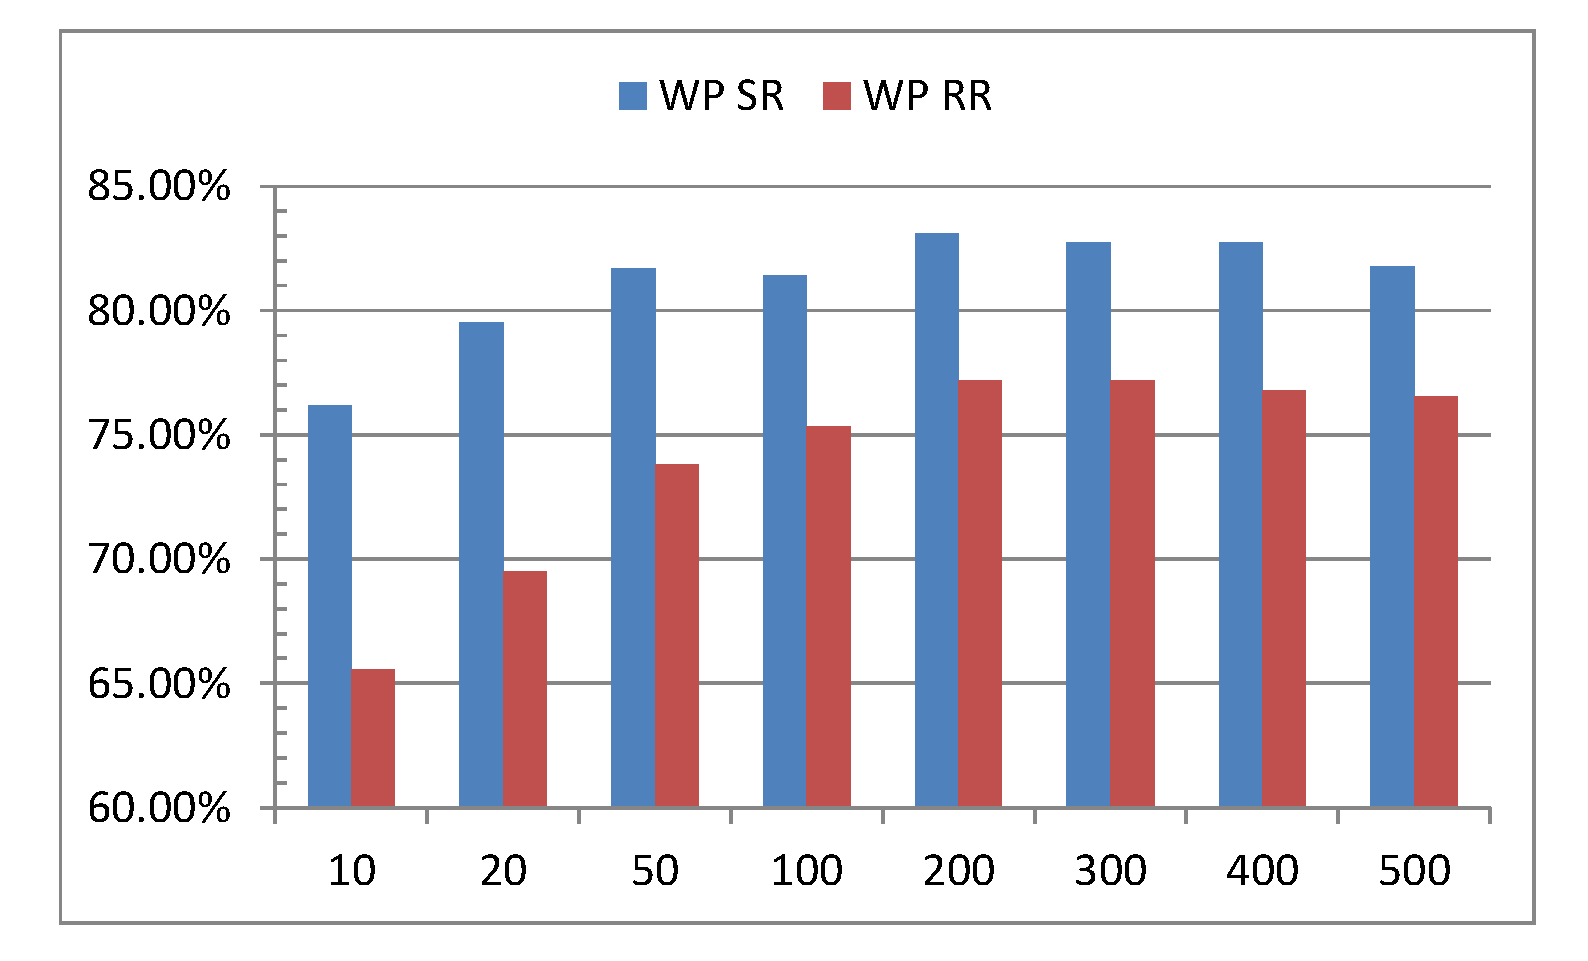
\includegraphics[width=1\linewidth]{num_letter_impact}
\vspace{-20pt}
\captionof{figure}{The impact of increasing the maximal number of samples per class on the segmentation and recognition rates. }
\end{center}

}

\end{poster}

\end{document}

\end{poster}

\end{document}